% File: lab-report.tex
\documentclass[11pt]{article}

\usepackage[utf8]{inputenc}
\usepackage[spanish]{babel}
\usepackage[T1]{fontenc}

\usepackage{amssymb} % AMS fonts
\usepackage{amsmath}
\usepackage{amsthm}

\usepackage{../common/file-config}
\usepackage{../common/colours}
\usepackage{../common/listings-config}

\usepackage{graphicx}
% \graphicspath{{res/}}

% Tables
\usepackage{booktabs}
\usepackage[table]{xcolor}
\usepackage{multirow}
\usepackage{makecell}
\usepackage{tabularx}

% Images
\usepackage{rotating}

% Algorithms
\usepackage{algorithm}
\usepackage{algpseudocode}
\floatname{algorithm}{}
\renewcommand{\thealgorithm}{}

\usepackage{url}
\usepackage[pdftex, colorlinks=true, citecolor=cyan, linkcolor=black, 
urlcolor=blue]{hyperref}

\usepackage[backend=biber, style=numeric]{biblatex}
\addbibresource{references.bib}

\begin{document}
    
\begin{titlepage}
	\centering
    
\includegraphics[width=0.5\textwidth]{../logo/logo_rw.jpg} 

		08 -- Roberta Williams 
\par \vspace{1cm}


	{\Large Contacto} \par
    %\texttt{NIP} \par
		\begin{table}[h]
				\centering
				\begin{tabular}{cl} 
						845977 & Jaime Alconchel Gallego \\ 
						844699 & Mario Casado Fontana \\
						842102 & Cristina Embid Martínez \\ 
						844472 & Hugo Naudín López \\ 
						844459 & Miguel Ángel Luquín Guerrero  \\ 
						792310 & Julia Quero Pérez  \\
						843740 & Nicolás Eugenio de Rivas Morillo \\ 
						844487 & Miguel Ángel Royo Miguel  \\
			\end{tabular}
		\end{table}
	\vspace{2cm}
	{\huge\bfseries Plan de gestión, análisis, diseño y memoria del proyecto\par}
    
\includegraphics[width=0.9\textwidth]{../logo/logo.png} \par \vspace{1cm}
    \vfill
    {\Large \today \par}
\end{titlepage}

% \clearemptydoublepage

\thispagestyle{empty}
\tableofcontents

\newpage
% \clearemptydoublepage

\section{Introducción} % TODO JULIA
El presente documento recoge el plan de gestión, análisis, diseño y memoria
del proyecto Magnate.
Magnate es un sistema 
que consiste en un juego multiplataforma, para escritorio
y web, online y multijugador, con funcionalidades de tipo de red social.
Tendrá un diseño sencillo, estético y lúdico. 
Magnate es un juego de mesa por turnos basado en el
popular juego Monopoly, tomando inspiración adicional de la saga de 
videojuegos Mario Party. Magnate busca ser un juego dinámico con alto grado
de aleatoriedad, pero sin perder la estrategia del Monopoly original,
al que añade más reglas que esperan hacer de la 
experiencia de juego novedosa y emocionante.
Estas incluyen un tablero en dos niveles, un nuevo sistema de tarjetas,
más formas de desplazamiento a lo largo del tablero y un nuevo sistema de
puntuación.

El sistema permitirá dos modos de juego: partidas online y
partidas locales. Las partidas online se realizarán en salas públicas con 
4 usuarios interesados en jugar partidas online. Las partidas locales
permitirán el juego de varios jugadores en local y bots, sumando hasta
4 jugadores. 

Los principales objetivos del sistema, ordenados según los hitos de desarrollo,
son los siguientes:
\begin{itemize}
		\item El sistema permitirá jugar a Magnate, un juego que incorpore
				a las mecánicas habituales del Monopoly nuevas reglas de
				desplazamiento y acumulación de efectos, y que será 
				dinámico, aleatorio, divertido y fácil de usar.
		\item Las partidas podrán pausarse y reanudarse entre dispositivos.
		\item El sistema permitirá asociar cuentas de usuario con la 
				información de las partidas y características de red social.
		\item Desarrollar un sistema de emparejamiento para las partidas
				online.
		\item Implementar bots que jueguen a Magnate con usuarios en local.
		\item El juego ofrecerá una experiencia atractiva y personalizable,
				incluyendo una tienda de cosméticos.
		\item Garantizar la seguridad y privacidad de los usuarios.
\end{itemize}

El sistema será compatible con el navegador web Chromium 144.0.7559.96 y
para aplicaciones de escritorio con el sistema operativo Arch Linux 6.18.6.
Se desplegará en varios 
contenedores Docker en un servidor de la empresa 08 -- Roberta Williams.
Las tecnologías a utilizar abarcan Godot 4.6, React, Django y PostgreSQL.

El desarrollo del sistema se realizará a lo largo de los meses de febrero,
marzo, abril y mayo. Los hitos principales son:
\begin{itemize}
		\item 10 de abril. Demostración de una primera versión funcional del
				sistema con la jugabilidad básica del juego y
				tratamiento básico de los usuarios. (RF)
		\item 4 o 5 de mayo. Presentación del producto a los clientes.
		\item Semana del 11 de mayo. Demostración del juego completo
				desplegado con todas las funcionalidades especificadas.
		\item 27 de mayo. Entrega del Plan de gestión, análisis y diseño y
				memoria del proyecto. Entrega del código al cliente.
				Cierre del proyecto.
\end{itemize}

El precio del sistema y el proyecto suman 30795,50 €. 
Por dicho precio se entregará lo siguiente a la finalización del proyecto:
\begin{itemize}
		\item Todo el código desarrollado.
		\item Documentación de despliegue y ficheros de configuración y Docker Compose para el despliegue.
		\item El presente documento. 
		\item Un exec con la versión escritorio.
\end{itemize}

Los apéndices incluyen 
la sección \ref{sec:glosario}, que recoge las abreviaciones utilizadas
en el documento; y
la sección \ref{sec:reglas}, donde se detallan las reglas del juego Magnate.

\newpage

\section{Organización del proyecto}
\label{sec:equipo}
Los encargados del proyecto son la totalidad de la empresa 08 -- Roberta Williams, que conformamos los estudiantes de
5º curso del Programa Conjunto en Matemáticas e Ingeniería Informática de la Universidad de Zaragoza. 
La conformación del equipo de trabajo surge de manera natural tras las experiencias compartidas a lo
largo del grado, que refuerzan nuestra confianza y seguridad en nosotros mismos como equipo y como
profesionales. 

Basándonos en nuestras habilidades y experiencia previa, se ha decidido conjuntamente el siguiente 
reparto de cargos y tareas principales, 
recogido en la Tabla \ref{tab:cargos}.

\begin{table}[h]
		\centering
		\begin{tabular}{|l|c|c|c|c|c|}
				\hline
				\textbf{Hugo}
& \multirow{5}{*}{backend} 
& 
& IA 
& apoyo docu. 
& \\ \cline{1-1}\cline{3-6}

				\textbf{Jaime} 
& 
& \multirow{3}{*}{despliegue} 
& \makecell{encargado\\despliegue}
& apoyo docu. 
& \makecell{coordinador\\backend} \\ \cline{1-1}\cline{4-6}

				\textbf{Mario}
& 
& 
& \makecell{lógica del\\juego}
& \multirow{4}{*}{\makecell{diseño de\\marca}} 
& \\ \cline{1-4} \cline{6-6} 

				\textbf{Miguel Royo}
& \multirow{10}{*}{frontend} 
& \multirow{5}{*}{web} 
& \makecell{coordinador\\frontend}
& 
				& \multirow{3}{*}{\makecell{diseño\\interfaz}} \\ \cline{1-1} \cline{4-5}

				\textbf{Cristina}
& 
& 
& \makecell{encargada\\calidad web}
& apoyo docu. 
& \\ \cline{1-1}\cline{4-6}

				\textbf{Julia} 
& 
& 
& calidad 
& documentación 
& \makecell{gestión del\\proyecto} \\ \cline{1-1}\cline{3-6}

				\textbf{Nicolás} 
& 
& \multirow{4}{*}{escritorio} 
& \makecell{encargado\\escritorio}
& apoyo docu. 
& \multirow{4}{*}{\makecell{diseño\\interfaz}}\\ \cline{1-1}\cline{4-5}

				\textbf{Miguel Luquín} 
& 
& 
& \makecell{encargado\\calidad\\escritorio}
& diagramas 
&  \\ 
				\hline
		\end{tabular}
		\caption{Relación de cargos y tareas principales en la empresa 08 -- Roberta Williams.}
		\label{tab:cargos}
\end{table}

De los roles recogidos en la Tabla \ref{tab:cargos}, queremos
destacar las siguientes responsabilidades:
\begin{itemize}
\item Directora de proyecto: Julia Quero Pérez
\item Coordinador de fronend: Miguel Ángel Royo Miguel
\item Coordinador de backend: Jaime Alconchel Gallego
\item Coordinadora de calidad: Cristina Embid Martínez
\item Coordinador de despliegue: Jaime Alconchel Gallego
\end{itemize}

% PREGUNTAR ¿tengo que detallar más cada tarea?
% Aunque no sea por cada uno, por "desarrollador web" tal vez, aunque para
% eso prefiero hacerlo para cada uno...

\section{Plan de gestión del proyecto}
\label{sec:plan}
En esta sección se describe cómo se llevarán a cabo los distintos procesos o
tareas a realizar a lo largo del tiempo, su temporalidad, los recursos a
emplear y quién son sus responsables.

\subsection{Inicio del proyecto} % htas y metodología
Se ha priorizado el uso de herramientas abiertas o de software libre para la
realización del proyecto, por lo que los recursos materiales y software 
se reducen a los ya accesibles a los miembros del equipo. Estos incluyen los
ordenadores portátiles de cada miembro del equipo y el servidor que posee
Mario.

La formación inicial necesaria para los miembros del equipo, por tecnología
utilizada, se detalla a continuación:
\begin{itemize}
		\item Godot 4.6 (implementación del sistema para aplicación de escritorio): Miguel, Miguel y Nicolás buscarían por su cuenta tutoriales de la aplicación.
		\item React (implementación del sistema para navegador web): Miguel Royo buscaría información al respecto, y Cristina le ayudaría a buscar tutoriales y proyectos de la librería Phaser para el juego.
		\item Django (backend): Los miembros del equipo ya tenían experiencia con la tecnología.
		\item PostgreSQL (gestor de BDD): Los miembros el equipo ya tenían
				experiencia con la tecnología.
\end{itemize}

\subsubsection{Mitigación de riesgos}
Se han detectado los siguientes riesgos del proyecto:
\begin{itemize}
		\item[Ri1] Hay integrantes del equipo que tienen muchos proyectos (y/o asignaturas a la vez).
		\item[Ri2] La falta de experiencia trabajando juntos puede afectar al éxito del proyecto.
		\item[Ri3] La toma de decisiones se puede bloquear por no estar dispuestos los miembros del equipo a asumir las responsabilidades.
		\item[Ri4] Nunca se ha trabajado en un grupo tan grande.
		\item[Ri5] El desconocimiento del cliente.
		\item[Ri6] El proyecto cuenta con unas funcionalidades que no están muy claramente definidas.
		\item[Ri7] Nunca se ha construido un sistema tan complejo como el propuesto.
		\item[Ri8] Se ha elegido una tecnología que se conoce poco o nada.
		\item[Ri9] Se ha trabajado, o no, con el entorno de despliegue elegido.
		\item[Ri10]La fecha de entrega está muy lejos en el tiempo.
		\item[Ri11]El proyecto hay que desarrollarlo en dos fases.
\end{itemize}

Para ellos se proponen las siguientes estrategias de mitigación:
\begin{itemize}
		\item[Ri1] Promover la organización individual, evitar el solapamiento en la definición de las tareas y fijar fechas internas para todas las pequeñas tareas. Responsables: Julia, Cristina.
		\item[Ri2] Favorecer la comunicación inmediata en los grupos de WhatsApp y Discord. Responsable: Julia.
		\item[Ri3] Repartir las tareas conforme surgen. Responsables: Julia, Jaime y Miguel Royo.
		\item[Ri4] Fomentar el uso de herramientas y metodologías para la comunicación fluida (WhatsApp, Discord), realizar un reparto de trabajo a nivel
				de los grupos de trabajo y posteriormente ponerlo en común y
				conjunto en las sesiones de prácticas con el equipo al completo. Responsables: Julia, Jaime y Miguel Royo.
		\item[Ri5] Aprovechar las sesiones de prácticas para consultar el estado del proyecto y solicitar retroalimentación. Responsable: Julia.
		\item[Ri6] Establecer requisitos claros. Responsable: Julia.
		\item[Ri7] Dividir el proyecto en tareas pequeñas y autocontenidas por equipos y establecer fechas para juntar los resultados. Responsable: Julia.
		\item[Ri8] Fomentar la consulta y realización de tutoriales al
				comienzo del proyecto, previo al desarrollo.
				Responsable: Miguel Luquín.
		\item[Ri9] Revisar proyectos ya realizados con esa misma tecnología y
				hacer alguna prueba menor antes de configurar el sistema
				completo. Responsable: Jaime.
		\item[Ri10]Poner fechas internas con un margen suficiente para entregar a tiempo el proyecto en las fechas de entrega con el cliente. 
				Responsable: Julia.
		\item[Ri11]Establecer fechas intermedias (hitos en Github issues).
				Responsables: Cristina, Nicolás, Mario.
\end{itemize}

\subsection{Control de configuraciones, construcción del software y aseguramiento de la calidad del producto}
Las \textbf{herramientas} a utilizar en el proyecto se han elegido por ser
aquellas que aportan más profesionalidad y por contar cada miembro con
experiencia en su uso.

El código del proyecto se ha desarrollado en el entorno de desarrollo
(VisualStudio Code o vim) de la preferencia de cada integrante, y se ha
integrado en la plataforma GitHub, utilizando
la herramienta git de control de versiones, así como la documentación
escrita con LaTeX. 

Adicionalmente se ha utilizado la plataforma de gestión
de archivos Google Drive y sus filiales Google Sheets y Google Docs para 
el seguimiento del desempeño, la realización de presupuestos o análisis
y compartir de forma preliminar cierta información bibliográfica o de gestión.
Para la creación de diagramas arquitecturales se ha seguido la notación
UMLS, y se ha utilizado % TODO LUQUIN
Para los diagramas de tareas, por otro lado, se ha utilizado una hoja de cálculo de Google Sheets.
Para el diseño de la GUI, por un lado se concretó una guía de estilo general
de los elementos de la interfaz, y posteriormente se realizan a papel los
bocetos de cada pantalla, que tienen su primer prototipo directamente en la
tecnología escritorio o web utilizada en el proyecto. Los diseños se hacen
siguiendo el sentido estético del equipo de frontend, más desarrollados por
algunos de sus miembros que otros, que se centran en las cuestiones de 
usabilidad. Como referencia para la interfaz se siguen Las 8 reglas de oro
de Schneiderman, y se intentan minimizar la interacción del usuario sin
comprometer su comprensión. En el diseño estético se eligieron un
número reducido de colores principales y secundarios y se consensuaron los
formatos de los elementos básicos (botones, fondos...) para la consistencia.

Por último, las herramientas de despliegue engloban
% TODO @BACKEND Htas despliegue alguien de backend porfa

Los \textbf{responsables} de supervisar la corrección de las configuraciones,
construcción del software y calidad del producto son para el código del
backend Jaime (el coordinador del backend) y para el código del frontend
Miguel (el coordinador del frontend).

La convención de nombrar ficheros y documentos y 
\textbf{estándares de código} %TODO JAIME TODO MIGUEL TODO NICO
% también mencionar qué herramientas lo pueden sacar de forma automática
Clases con CamelCase y el resto con snake\_case.

El código se ha organizado en 4 \textbf{repositorios} de GitHub: uno para el backend,
otro para el frontend del cliente web, otro para el frontend del cliente 
escritorio y otro para la gestión y documentación. Todos los miembros del
equipo tienen acceso a todos los repositorios, y respetan el workflow
consensuado en el equipo. 
Las issues se crean tras una reunión entre los miembros del equipo 
correspondiente en la que se identifican, definen y reparten las tareas a
realizar. Se designa un encargado que cree en Github las issues 
correspondientes. Para realizar un commit en el repositorio compartido, se
ha de obtener el permiso de los demás usuarios habituales del repositorio
(los miembros del equipo correspondiente) para minimizar las posibles 
incongruencias (aunque ya se definen las tareas teniendo esto en cuenta), y
no se han de revisar los commits ya que se confía en la capacidad y buen
criterio de los miembros del equipo.

Ante la detección de \textbf{incidencias}, el que la haya detectado tiene la
responsabilidad de encontrar a la persona que haya generado la incidencia,
que llamaremos a partir de ahora el incidente. Será responsabilidad del
incidente decidir el plan de actuación para solventar la incidencia, en tanto
a si puede ser el único responsable y si es más prioritario o no que el
trabajo actual que haya que realizar.

% otras cosas de pruebas: rellenar con lo dicho en la p3 
Las actividades de \textbf{control de calidad} serán variadas. 
Se realizan pruebas por separado de frontend y backend y posteriormente se
realizarán pruebas de la conjunción de ambos.
Para las pruebas del backend se cuenta en primera instancia con test para
comprobar el correcto funcionamiento de las funciones. Para probar el juego
completo, se propone:
\begin{enumerate}
		\item Probar todos los arcos del grafo de juego forzando los escenarios correspondientes y eliminando el azar.
		\item Simular partidas con dos agentes jugando entre ellos.
\end{enumerate}
Para las pruebas del frontend, 
\begin{enumerate}
		\item En primera instancia, se comprobará manualmente la correcta inclusión del código en el sistema existente. 
		\item Se documentará mínimamente las entradas y salidas esperadas
				para la interacción con el juego (tirada de dados,
				compra de propiedad, pago de alquiler...) y se comprobará
				sistemáticamente la corrección del cliente correspondiente.
\end{enumerate}
Para el código a alto nivel, se contrastará con el
diagramador y los autores del código correspondiente que el comportamiento
del sistema coincide con lo expresado en el diagrama.
% scripts automatización NO, HACER COMO QUE NO EXISTEN

% cómo se hará la entrega de resultados al cliente % TODO JAIME CHECK
Se entregará al cliente lo siguiente a la finalización del proyecto:
\begin{itemize}
		\item Todo el código desarrollado.
		\item Documentación de despliegue y ficheros de configuración y Docker Compose para el despliegue.
		\item Un executable con la versión escritorio.
\end{itemize}


\subsection{Calendario del proyecto, división del trabajo, coordinación, comunicaciones, monitorización y seguimiento}
La responsable del calendario del proyecto, coordinación, y comunicaciones es 
Julia, la directora del proyecto,
apoyada en los coordinadores backend y frontend para una mejor descripción y
ordenación de las tareas, la división del trabajo y la monitorización y 
seguimiento de las tareas.

% Lo de las issues lo puse en 3.2 porque no sé qué son las incidencias

Para la \textbf{comunicación interna}, se han creado grupos de WhatsApp por proyecto
y por equipios, así como un canal de Discord análogo para comunicaciones y
cuestiones de rápida resolución o inmediatas, y se realizarán reuniones de 
seguimiento entre todos los equipos durante las sesiones de prácticas, así
como las reuniones dentro del equipo cuando los miembros lo estimen
oportuno. Las reuniones de las sesiones de prácticas servirán para
actualizar los planes en caso de desviarse del inicial. 
Las decisiones tomadas acabarán reflejadas en Github issues o en la 
documentación (o en la carpeta compartida de Drive a modo de borrador, 
de ser algo extenso, de forma provisional hasta aparecer en la documentación), 
por lo que no se utilizan documentos adicionales con actas.

Ante diferencias en la \textbf{gestión del equipo humano}, se plantea la 
inclusión de
mediadores imparciales o no involucrados en la disputa inicial para intentar
consensuar a las partes. En caso de no resolverse el conflicto, se pospondrá
la discusión a cuando se halla enfriado, no siendo más de 2 semanas.

\begin{sidewaysfigure}[hbtp]
\centering
		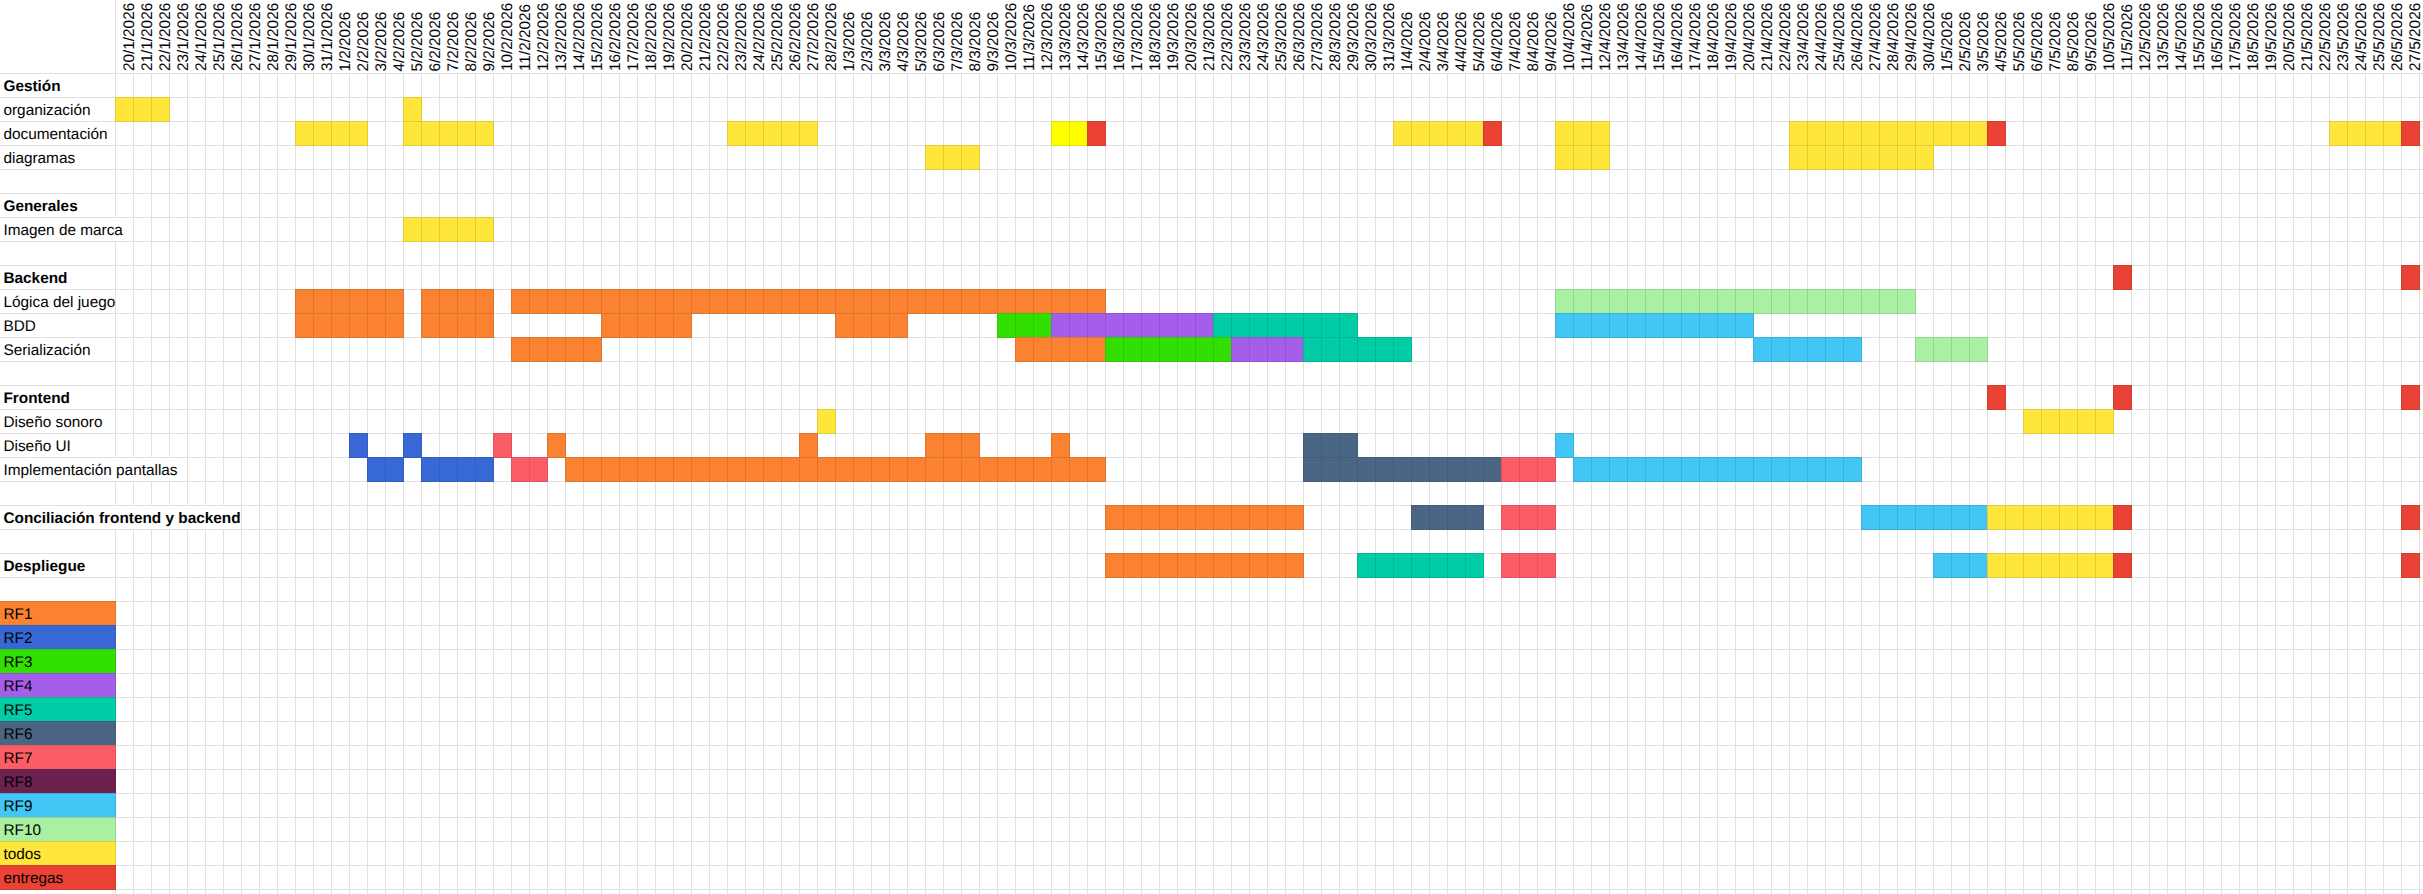
\includegraphics[width=\textwidth]{img/gantt.png}
		\caption{Diagrama de Gantt con la planificación del proyecto.}
		\label{fig:gantt}
\end{sidewaysfigure}


Para la \textbf{monitorización y medición del progreso}, 
cada lunes y viernes se
revisarán las tareas realizadas por los miembros del equipo correspondiente.
Se mira la consecución de la tarea, y de haber quedado mucho por realizar,
dado que confiamos en el buen trabajo de los miembros del equipo, concluiremos que el retraso se ha debido a un reparto no equitativo y se volverá a
repartir la tarea faltante entre los miembros del equipo, para realizarse en
esa semana, antes que las tareas de dicha semana. 

Se ha intentado realizar
un plan lo suficientemente holgado como para que estas desviaciones, de no
prolongarse durante más de una semana, no supongan un problema.
De darse continuadamente este retraso, a una semana vista de la entrega se
replantearán las tareas a realizar, minimizando estas.

Sobre el \textbf{reparto y definición de tareas}, primero se ha realizado una
planificación global por requisitos como expresado en el diagrama de Gantt de
la Figura \ref{fig:gantt}. Para ello, se ha entendido que las etapas de 
calidad se producirán cada vez que se suba código a los repositorios y se ha
planificado un diseño iterativo y gradual por requisito.
A más bajo nivel, estas se
realizarán después de la monitorización del progreso, listando el desglose de
tareas necesarias para consecuir los objetivos semanales correspondientes al
diagrama de Gantt de la Figura \ref{fig:gantt}. 
Una vez se hayan desglosado las tareas y concordado
cómo se van a realizar (todo aquello que suponga cohesión, como interfaces
consistentes o comunicación entre elementos), se repartirán entre los miembros
del equipo, primando la equidad, los conocimientos y habilidades de
los miembros, y sus preferencias. Cada uno informará de sus preferencias y al
llegar al consenso entre todos se fijarán las tareas con su responsable como
Github issues.

\newpage

\section{Análisis y diseño del sistema}
En esta sección se detallan los requisitos y diseño del sistema.

\subsection{Análisis de requisitos}
En la Tabla \ref{tab:rf} se recoge la relación de requisitos funcionales del
sistema, y en la Tabla \ref{tab:rnf} se recogen los requisitos no
funcionales del sistema.
\begin{table}[htbp]
		\centering
\begin{tabularx}{\textwidth}{|l|X|l|}
		\hline
		ID & Descripción & Prioridad \\
		\hline
		RF-1.1 & 
		El sistema permitirá jugar a Magnate, siguiendo las reglas descritas
		en el Apéndice \ref{app:normas}. &
		M \\
		\hline
		RF-1.2 &
		El sistema mostrará los resultados de una partida una vez finalizada, incluyendo el capital final de los jugadores y los beneficiarios de los bonus finales aplicados. &
		M \\
		\hline
		RF-2.1 &
		El sistema debe permitir a los usuarios registrarse con un nombre de usuario único y una contraseña. 
		& M \\
		\hline
		RF-2.2 &
		El sistema exige para el registro de una cuenta de usuario nueva que se confirme la contraseña.
		& M \\
		\hline
		RF-2.3 &
		El sistema debe permitir a los usuarios iniciar sesión introduciendo su nombre de usuario y su contraseña.
		& M \\
		\hline
		RF-3 &
		El sistema guardará la información de las partidas en curso necesaria
		para reanudarlas.
		& M \\
		\hline
		RF-4.1 &
		El sistema almacenará el historial de partidas de los usuarios.
		& M \\
		\hline
		RF-4.2 &
		El sistema permitirá a los usuarios consultar su historial de partidas completas.
		& M \\
		\hline
		RF-4.3 &
		El historial de partidas recogerá para cada partida la posición en
		la que quedó el usuario tras jugarla y las monedas que ganó.
		& M \\
		\hline
		RF-5 &
		Las partidas se pueden pausar y reanudar en otra plataforma.
		& M \\
		\hline
		RF-6.1 &
		El sistema permitirá a los usuarios que hayan iniciado sesión observar su propia información ligada a un usuario.
		& M \\
		\hline
		RF-6.2 &
		La información ligada a un usuario incluye: nombre de usuario, skin de ficha predeterminada para jugar y estadísticas de sus partidas.
		& M \\
		\hline
		RF-6.3 &
		Las estadísticas de las partidas ligadas a un usuario incluyen: nº partidas jugadas, nº partidas vencidas, monedas para la tienda.
		& M \\
		\hline
		RF-6.4 &
		El sistema permitirá al usuario elegir su skin de ficha predeterminada entre las que posea.
		& M \\
		\hline
		RF-7.1 &
		El sistema permite jugar partidas en dos modalidades: partida pública y partida privada.
		& S \\
		\hline
		RF-7.2 &
		Las partidas privadas permitirán que jueguen los poseedores de un código de la sala privada y/o con bots, sumando hasta 4 jugadores.
		& S \\
		\hline
		RF-7.3 &
		Las partidas públicas realizan un emparejamiento entre los usuarios por orden de llegada, agrupando 4 jugadores siempre que haya suficientes en línea.
		& S \\
		\hline
		RF-7.4 &
		La moneda del juego se recibe tras jugar cada partida como el capital remanente al terminar la partida y aplicar los bonus.
		& S \\
		\hline
		RF-8.1 &
		El sistema permitirá a los usuarios intercambiar mensajes en lenguaje natural durante el transcurso de una partida.
		& C \\
		\hline
		RF-8.2 &
		El sistema permitirá a los usuarios incluir emoticonos en los mensajes del chat durante el transcurso de una partida.
		& C \\
		\hline
		RF-9.1 &
		Se pueden adquirir distintos skins para las fichas del juego en la tienda.
		& S \\
		\hline
		RF-9.2 &
		El sistema permitirá a los usuarios adquirir distintos skins para las fichas de las partidas de Magnate en la tienda, intercambiando la moneda del juego, que se obtiene jugando partidas.
		& S \\
		\hline
		RF-9.3 &
		Se pueden adquirir distintos emoticonos para emplear en el chat del juego en la tienda.
		& C \\
		\hline
		RF-9.4 &
		El sistema permitirá a los usuarios adquirir distintos emoticonos para el chat de las partidas de Magnate en la tienda, intercambiando la moneda del juego, que se obtiene jugando partidas.
		& C \\
		\hline
		RF-10 &
		Se diseñará una IA o bots contra la que jugar en las partidas privadas.
		& C \\
		\hline

\end{tabularx}
		\caption{Requisitos funcionales del sistema.}
		\label{tab:rf}
\end{table}

\begin{table}[hbtp]
		\centering
\begin{tabularx}{\textwidth}{|l|X|}
		\hline
		RNF-1 &
		El cliente de escritorio debe funcionar en un computador con sistema operativo Arch Linux 6.18.6.
		\\
		\hline
		RNF-2 &
		El cliente web debe funcionar en un navegador con versión Chromium 144.0.7559.96.
		\\
		\hline
		RNF-3 &
		El sistema es seguro a usos malintencionados de las plataformas.
		\\
		\hline
		\end{tabularx}
		\caption{Requisitos no funcionales del sistema.}
		\label{tab:rnf}
\end{table}
\subsection{Diseño del sistema} 
% TODO LUQUIN diagramas

% decisiones de diseño
\subsubsection{Decisiones de diseño}
Las primeras decisiones de diseño se tomaron sobre las \textbf{tecnologías}
a usar en el proyecto.
Para las tecnologías web se barajaron html con css y React. Aunque los
miembros del equipo tenían experiencia con html y css, la dificultad de 
realizar un proyecto tan complejo en estos lenguajes nos llevó a decidirnos
por React, cuya curva de aprendizaje es bastante menor una vez conocidas
estas tecnologías, y cuenta con una forma fácil de incluir paquetes de
componentes. Además, React cuenta con numerosas librerías sobre las que 
construir un juego. Se desestimó la librería para juegos boardgame.io ya
que esta supliría el trabajo del que se encarga el backend,
pero sí se utilizó Phaser para gráficos, componentes y elementos del juego, 
ya que tras dos días en los que Cristina y Miguel
sopesaron la decisión de utilizarla descubrieron que el aprendizaje merecería
la pena para el trabajo futuro a ahorrarnos.

Como segundo cliente se decidió el escritorio sobre el móvil porque 
facilitaría las labores de interfaz, al no tener que conciliar diseños
horizontales y verticales, y porque la tecnología para el desarrollo móvil
Android Studio ya era conocida por los miembros del equipo y se negaban a
volver a utilizarla. Así que como nueva tecnología para el escritorio se
optó por Godot, que tiene una interfaz para el desarrollo intuitiva y cuenta
con portabilidad a una amplia gama de dispositivos, por lo que se presentaba
como una buena herramienta para aprender.
% TODO JAIME alguna más propuso para escritorio, por nombrarla

Como tecnologías de backend se barajaron Django, Flask, NextJS y FastAPI, y se
decidió usar Django por tener experiencia previa en la tecnología y tener
todas prestaciones similares. Para la representación de la información se
utilizan ficheros JSON por su uso extendido y generalizado.
% TODO JAIME o alguien de backend en verdad no me enteré jajajajjaj

Para la base de datos, por motivos similares, se decidió la versátil y
básica base de datos SQL PostgreSQL.

% TODO decisiones sobre el diseño de la arquitectura, if any

\section{Memoria del proyecto} % TODO JULIA
En este capítulo se describe el ajuste a la realidad de lo previsto en
el plan de la Sección \ref{sec:plan}.
% comparar lo propuesto en el apartado 3 con lo que hemos hecho de verdad
\subsection{Inicio del proyecto} % 3.1 

\subsection{Ejecución y control del proyecto} % 3.2 y 3.3

\subsection{Cierre del proyecto} % vibes de conclusiones pero más curro

%\section{Conclusiones} % Solo para la entrega final...
%personales, mejorar los procesos... si no nos quejamos nos pone un 0

\newpage

\appendix

\section{Glosario}
\label{sec:glosario}

%\section{Resultados de la revisión intermedia}

%\section{Presentación final}
% copia de las transparencias y explicar cómo ha tenido en cuenta lo visto
% en teoría de cómo hacer presentaciones

\section{Análisis de riesgos}
En la Figura \ref{fig:riesgo} se recoge el análisis de riesgos detallado
realizado por la empresa.

\begin{sidewaysfigure}
		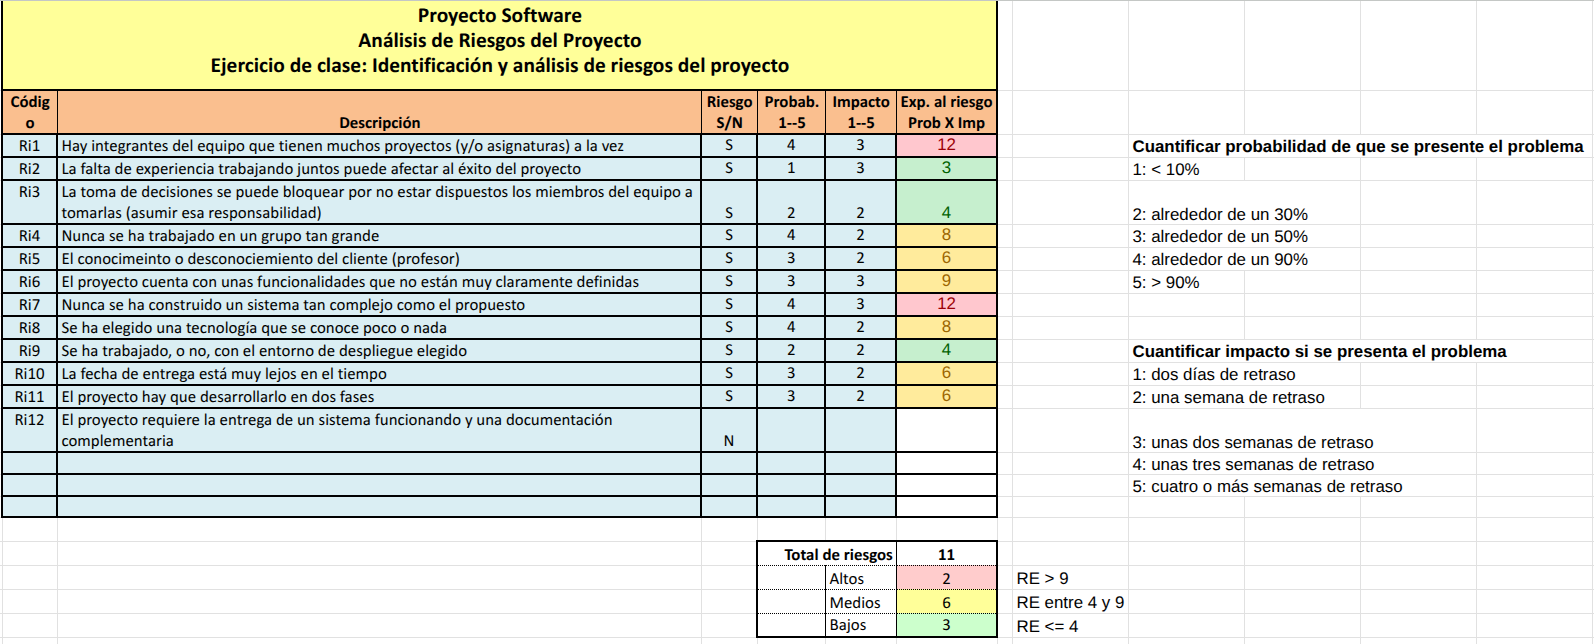
\includegraphics[width=\textwidth]{img/riesgos.png}
		\caption{Análisis de riesgos.}
		\label{fig:riesgo}
\end{sidewaysfigure}

\newpage

\section{Reglas}
\label{app:normas}
\subsection{Introducción}
En este documento se definirán las mecánicas y reglas del juego \textit{Magnate}.
Se explicarán las diferentes fases del juego, las acciones que pueden realizar 
los jugadores y las condiciones de victoria. 

Se definirá desde el diseño del tablero hasta los distintos eventos especiales
que pueden ocurrir, considerando todos los casos posibles.

Las reglas están basadas en las reglas originales del Monopoly \cite{hasbro_monopoly_es} 
tomando inspiración adicional de la saga de videojuegos Mario Party.
Magnate busca ser un juego dinámico con alto grado de aleatoriedad, pero
sin perder la estrategia del Monopoly original.

\subsection{Objetivo del juego}
El objetivo del juego es ser el jugador con mayor valor neto al final de la
partida, limitada por un número de rondas. El valor neto de un jugador se calcula
mediante la suma de su dinero en efectivo más el valor de venta
de todas sus propiedades, sin contar las que tenga hipotecadas y
el valor de venta de sus construcciones.



\subsection{Equipamiento}
A continuación está la lista de elementos para una partida.
\begin{itemize}
	\item Tablero
	\item 2 Dados normales
	\item 1 Dado bus 
	\item Cartas de las propiedades 
	\item Casas
	\item Hoteles 
	\item Cartas "Sales de la cárcel"
	\item Cartas de evento fantasía
\end{itemize}

\subsubsection{Los dados: definición y funcionamiento}
En el juego hay 3 dados en juego, 2 normales de 6 caras numerados del 1 al 
6 y uno especial llamado \textit{Dado bus}. El Dado bus está compuesto de 6
caras, 3 de ellas con el dibujo de un bus y las otras 3 numeradas del 1 al 3.

En una tirada de dados se tiran siempre los 3 dados a la vez.
En caso de salir 3 números se tendrá en cuenta para el movimiento
la suma total de los 3. En caso de salir un bus el jugador podrá elegir 3
valores: el valor de uno de los dados normales, el valor del otro de los dados
normales o la suma de los 2 dados normales.

Para las mecánicas de los dobles se tendrán en cuenta únicamente los dados 
normales. Al sacar dobles, el jugador gana una tirada extra. Si llega a 
sacar dobles una tercera vez consecutiva en el mismo turno, va directamente 
a la cárcel. 

Si en la tirada sale un triple (en los casos en los que el Dado bus saque número),
el jugador puede viajar a la casilla del tablero que quiera, aplicándose el efecto
de caer en esa casilla tal y como hubiera sido si la tirada hubiera sido 
convencional. Después de sacar un triple no se vuelve a tirar (como si de unos 
dobles se tratara). Los triples no cuentan en la racha de dobles, por lo que no 
te pueden mandar a la cárcel.

\subsubsection{Tablero}
El tablero está compuesto de 2 pistas cuadradas concéntricas:
el anillo exterior tiene 36 casillas y 4 esquinas y el anillo 
interior tiene 12 casillas y 4 esquinas. La particularidad
de las casillas para transición y cómo afectan al tablero 
se comentará con las casillas de puentes.


\subsection{Casillas}
En esta sección se definirán todos los distintos tipos de casilla 
que hay en el tablero y sus efectos y mecánicas.

\subsubsection{Propiedades}
Las propiedades son casillas que se pueden comprar, vender e hipotecar,
y por las que se cobra alquiler a jugadores rivales. Si un jugador 
cae en una de estas casillas pueden pasar varias cosas en función del 
estado de compra de la propiedad:
\begin{itemize}
	\item La casilla no tiene dueño. En este caso el jugador tiene derecho 
	a comprarla por el precio de compra indicado. En caso de no querer comprar o no 
	tener suficiente dinero, la propiedad pasa a ser subastada.
	\item La casilla tiene dueño. El jugador debe pagar el alquiler calculado
	en función de las construcciones o de si tiene el grupo completo.
	\item La casilla está hipotecada. No ocurre nada.
	\item La casilla es del propio jugador. No ocurre nada.
\end{itemize}

\subsubsection{Grupos de propiedades}
Las propiedades están divididas en grupos de color. Un jugador que posea
todas las propiedades de un mismo grupo, podrá cobrar el doble de alquiler
por las propiedades sin construcciones
y obtendrá derecho a construir en ellas.


\subsubsection{Puentes}
Los puentes son un tipo especial de propiedad. En el juego tienen
una función doble: poder ganar dinero por alquiler (como el resto de 
propiedades), y habilitar la transición entre el cuadrado interior y el 
cuadrado exterior.

El alquiler a pagar en los puentes viene marcado por el número de 
puentes que el jugador posea.

La mecánica de transición viene marcada por el valor usado 
en la tirada de dados (las casillas que el jugador elige mover). Si la 
tirada es par se continúa en el mismo cuadrado, si es impar se cambia de 
cuadrado (o viceversa, lo que indique la casilla).

En caso de caer justo en la casilla del puente, la decisión par o impar 
la tomará la tirada de dados de la siguiente jugada y no la tirada de la jugada 
de caer en el puente.

Las casillas puente, a pesar de ocupar el espacio de 2 casillas convencionales
únicamente contarán como una en los movimientos tanto en los casos de 
mantenerse en el cuadrado como en el caso de transicionar al otro
cuadrado.

\subsubsection{Servidores}
Los servidores son otro tipo especial de propiedad. El valor de su 
alquiler viene determinado por la cantidad de servidores que 
el jugador posea.

\subsubsection{Casillas fantasía}
Al caer en una casilla fantasía, aparecerán 2 cartas, una desvelada y 
una oculta. La carta desvelada tendrá un evento fantasía aleatorio, que se podrá 
aplicar por el precio indicado en la carta. El evento fantasía de la 
carta oculta es gratuito.
En caso de no querer comprar el evento desvelado, o no tener dinero 
para comprarlo, habrá que escoger la carta oculta obligatoriamente.
En caso de comprar y aplicar el evento fantasía de pago, no se aplicará 
ni desvelará el evento oculto.

Los eventos fantasía tendrán acciones positivas (como ganar dinero),
negativas (como perder propiedades) o neutras (como mover a otro 
jugador a cualquier casilla del mapa).

\subsubsection{Vas a la cárcel}
Si caes en esta casilla vas directamente a la cárcel y acaba tu turno.
En el caso de que el jugador deba dinero al banco se le permitirá realizar
las gestiones necesarias para saldar su deuda.

\subsubsection{Cárcel}
Un jugador en la cárcel tiene derecho al principio de su turno a 
tirar los dados. Si saca dobles puede salir de la cárcel usando 
el valor de la tirada y jugar su turno con normalidad (pero sin repetir turno por ser dobles).
Si no saca dobles, puede pagar una fianza de valor fijo. 
Si al tercer turno en la cárcel no ha 
salido, será obligado a pagar la fianza.

Los jugadores en la cárcel tienen derecho a cobrar alquileres y a realizar
acciones de gestión en su turno, pero no pueden moverse por el tablero ni
participar en las subastas.

Los turnos en los que un jugador acabe en la cárcel acaban cuando se 
entre en la cárcel sin tener oportunidad de hacer gestiones (excepto
el caso en el que tenga que saldar deudas con el banco).

\subsubsection{Salida}
En esta casilla comienza la partida y cada vez que un jugador pasa por
ella (al caer justo sobre ella o la primera tirada en la que la dejas atrás
de la vuelta al cuadrado correspondiente) 
recibe una cantidad fija de dinero. 

Si por algún motivo un jugador 
decide mantenerse en el cuadrado interior y no pasar por salida, no recibirá
dinero.

\subsubsection{Tranvías}
Hay 4 estaciones de tranvía repartidas por las esquinas del tablero. Si un 
jugador cae en una de estas casillas podrá moverse directamente a otra 
estación de tranvía de su elección pagando un precio por el desplazamiento.


\subsubsection{Párking}
Durante la partida, las multas, pagos de impuestos y demás ingresos 
a la banca en general,
se acumularán en un bote. El jugador que caiga en el parking se llevará
el bote completo. Si el bote está vacío, no ocurre nada.

\subsection{Preparación}
Cada jugador comienza con una cantidad de dinero determinada.
El turno se elige tirando un único dado, el que obtenga mayor valor empieza.
En caso de empate se vuelven a lanzar los dados para desempatar.
El orden de valores indica el orden de juego
de mayor a menor.


\subsection{Turno de juego}
Al comienzo del turno, el jugador lanzará los dados y moverá en función de lo 
que salga. Al caer en una casilla, se aplicará su efecto correspondiente.
Tras todos los efectos de casilla, el jugador podrá realizar acciones de 
gestión. Estas acciones son: comprar o vender construcciones, hipotecar o 
deshipotecar propiedades y comprar o vender propiedades a otros jugadores (intercambios, ver la Sección \ref{sec:intercambios}).

Haga lo que haga el jugador, su balance debe quedar positivo al final de su turno,
de lo contrario será declarado en bancarrota y eliminado de la partida.

\subsection{Subastas}
Las subastas serán pujas abiertas de valor oculto. Es decir, cada jugador
participante en la puja decidirá si participar o no, y en caso de participar
elegirá el valor por el que puja. El resto de jugadores no sabrá en ningún 
momento los jugadores que deciden participar en la puja ni los valores por los 
que pujan hasta el final de la subasta, donde se desvelarán los valores y 
el ganador de la puja. En caso de empate la propiedad no se dará a nadie.

Los jugadores que provocan una subasta no podrán participar en ella.

\subsection{Alquileres}
Si un jugador cae en una propiedad de otro jugador, deberá pagar el alquiler
correspondiente. El alquiler se calcula en función de si el dueño tiene el grupo 
de propiedades completo y de las construcciones que haya en la propiedad.

En caso de que el jugador no tenga dinero para pagar el alquiler al dueño,
el banco pagará el alquiler y al final del turno, el jugador deberá saldar 
su deuda con el banco mediante el hipotecado de propiedades o la venta de
construcciones o propiedades tanto al banco como a otros jugadores.

\subsection{Construcciones}
Una vez un jugador tiene el grupo completo de un color, podrá construir
casas en las propiedades de este grupo. El coste de construcción de cada 
casa vendrá marcado en cada propiedad. Las casas deben construirse de forma 
escalonada, es decir, si se quiere construir una segunda casa en una propiedad 
primero se tendrá que tener una casa en el resto de propiedades del grupo.

Una vez un jugador tenga 4 casas en todas las propiedades de un grupo, podrá
sustituir las 4 casas de una propiedad por un hotel por el precio de compra
de una casa.

A la hora de demoler construcciones se hará igualmente de forma escalonada en 
sentido inverso. En el caso particular de los hoteles, no se demolerán de golpe,
sino que primero se pasará de hotel a 4 casas.
El jugador recibirá la mitad del precio de compra de las construcciones demolidas.

\subsection{Intercambios}
\label{sec:intercambios}
Cada turno, el jugador podrá proponer intercambios a otros jugadores. Un 
intercambio se hará entre el jugador que lo propone y otro que podrá elegir.
Se podrán intercambiar dinero y cartas (propiedades, servidores y puentes)
por dinero y cartas. 

No se podrán intercambiar propiedades de un grupo de propiedades en el que
alguna de las propiedades tengan construcciones.

\subsection{Bonificaciones finales}
Al final de la partida, antes de desvelar al ganador, se aplicarán 3
bonificaciones finales aleatorias. Las bonificaciones darán una cantidad
de dinero determinada por un porcentaje del valor total de todos los jugadores 
sumado.
Estas bonificaciones vienen determinadas por estadísticas de la partida,
como el jugador que más se haya desplazado o el que más alquileres ha 
tenido que pagar al resto de jugadores, entre otras.

\subsection{Bancarrota}
Si un jugador no logra acabar su turno con balance positivo,
incluso después de hipotecar sus propiedades,
de vender todas sus construcciones y en general después de hacer 
gestiones para recaudar dinero,
todas las propiedades que le queden serán embargadas por el banco,
poniéndolas inmediatamente a la venta por su valor original.

Esto se aplicará también a los jugadores que se rindan, cuyo dinero en 
metálico quedará además absorbido por el banco sin ir al párking gratuito.





\end{document}
